\Needspace{.25\textheight}\subsection{Lectura comparada de la variabilidad}
El CV de calendario y el CV entre días activos responden a preguntas distintas. El primero compara los clics de todos los días observados, incluidos los ceros, y combina la ausencia de actividad con la variación de su intensidad. El segundo compara únicamente los días con clics y describe cuánto varía la intensidad cuando existe actividad. Por ello, un CV activo igual a cero puede coexistir con varios días sin interacción.

La Figura~\ref{editorial:cv} presenta cuatro secuencias hipotéticas de ocho días, correspondientes al calendario inclusivo del corte 7. Todas acumulan 40 clics; los cálculos utilizan desviación estándar muestral. Esta construcción permite aislar diferencias entre indicadores sin atribuirlas a cambios de volumen ni presentarlas como observaciones del estudio.
\begin{figure}[p]\centering
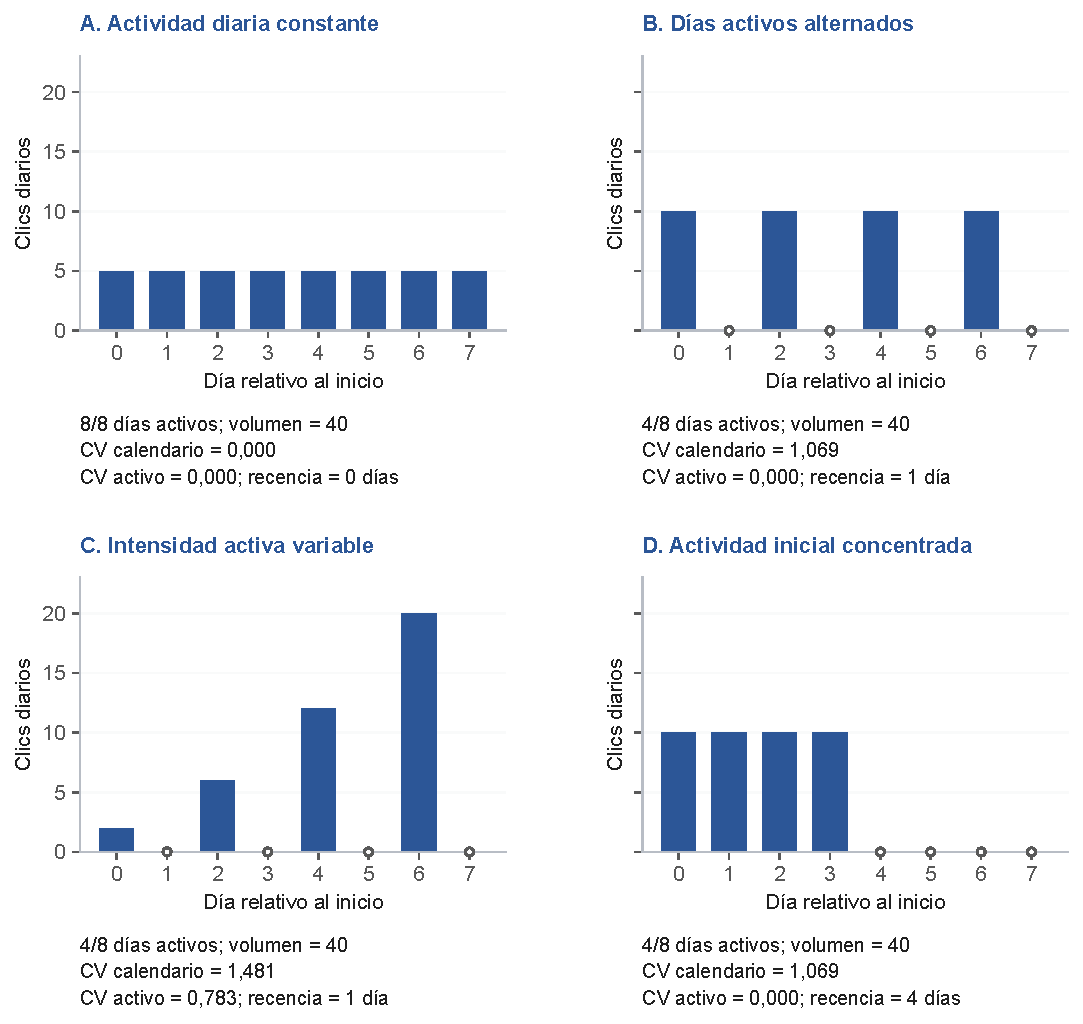
\includegraphics[width=.98\linewidth]{figuras_editoriales/comparacion_cv.pdf}
\caption{Comparación didáctica de los dos coeficientes de variación. Elaboración propia a partir de secuencias hipotéticas; los círculos sobre el eje indican días con cero clics.}\label{editorial:cv}
\end{figure}

En A se registran cinco clics todos los días y ambos CV son cero. En B se alternan días con diez clics y días sin actividad: el CV activo sigue siendo cero, pero el CV de calendario alcanza aproximadamente 1,069. Al comparar B con C se mantiene la misma cantidad de días activos; la intensidad deja de ser constante y aumentan ambos CV. Estos contrastes ilustran los dos componentes de la identidad~\eqref{corr:identidadcv}.

La comparación de B con D precisa otro límite: las secuencias contienen los mismos valores en distinto orden y, por tanto, producen los mismos CV. Sin embargo, la recencia cambia de uno a cuatro días. Los CV resumen dispersión y no identifican por sí solos el orden de la actividad; la recencia y las tendencias conservan información temporal complementaria. Ninguno de estos ejemplos establece una regla de abandono. Cuando todos los días tienen cero clics, ambos CV permanecen sin definición; cuando solo existe un día activo, no se calcula el CV activo muestral.
